% Application - Code
%%%%%%%%%%%%%%%%%%%%%%%%%%%%%%%%%%%%%%%%%%%%%

% FR
%\section{Développement de l'application}

% EN
\section{Application's Development}

% FR
% Pour obtenir un code efficace, maintenable et évolutif, il est nécessaire de devoir penser à la fléxibilité de celui-ci. En effet, plus il est possible d'ajouter des fonctionnalité, des outils et de personnaliser son environnement, plus l'outil est polyvalent.

% EN
For an efficient, scalable and maintainable code, it is necessary to have to think about the flexibility of it. Indeed, it is possible to add functionality, tools and customize its environment, the tool is more versatile.

%%%%%%%%%%%%%%%%%%%%%%%%%%%%%%%%%%%%%%%%%%%%%%%%%%%%%%%%%%%%%%%%%%%%%%%%%%%%%%

% FR
%\subsection{Environnement}

% EN
\subsection{Environment}

% FR
%Avant d'entamer le coeur du développement, il est nécessaire de rappeler l'environnement dans lequel l'application est développée. 

%L'application doit être utilisable sur un environnement web, sur bureau et sur mobile. De fait, l'application peut être consultable depuis un navigateur web. Il est également intéressant de penser dès maintenant à la protabilité vers une application mobile (Android, iOS, Windows Phone, FirefoxOS). Un code modulable est intéressant, mais encore plus s'il peut être adapté selon les plateformes désirées.

%Coté serveur, nous disposerons de toutes les informations cartographiques nécessaires. Pour celà, il faut pouvoir construire un serveur ouvert sur internet et pouvant répondre aux requêtes web venant de l'application.

%Les technologies choisies sont donc :

% \begin{description}

%   \item[Serveur] \hfill 
%     \begin{itemize}
%       \item Apache2 : Le logiciel libre Apache HTTP Server (Apache) est un serveur HTTP créé et maintenu au sein de la fondation Apache. Il servira de serveur Web.
%       \item Tomcat7 : Apache Tomcat est un conteneur web libre de servlets et JSP Java EE. Il servira à faire tourner les sources GéoServer.
%       \item GéoServer : GéoServer est un serveur informatique open source et libre écrit en Java qui permet aux utilisateurs de partager et modifier des données géographiques. Il contiendra nos informations cartographiques.
%       \item REST Services : Les services web de type Representational state transfer (REST) exposent entièrement des fonctionnalités comme un ensemble de ressources (URI) identifiables et accessibles par la syntaxe et la sémantique du protocole HTTP. Ce type de service est exécutée par un script Python en Deamon.
%     \end{itemize}

%   \item[Application] \hfill 
%     \begin{itemize}
%       \item HTML : L’Hypertext Markup Language, généralement abrégé HTML, est le format de données conçu pour représenter les pages web. 
%       \item CSS : Les feuilles de style en cascade est un langage informatique qui décrit la présentation des documents HTML et XML. Ce langage permettra de donner un style à notre application.
%       \item Javascript : JavaScript est un langage de programmation de scripts principalement employé dans les pages web interactives mais aussi pour les serveurs. Ce langage nous permettra de faire les interractions entre notre contenu HTML et nos données SIG contenu sur le serveur. Il permettra de gérer les interractions.
%     \end{itemize}

%   \item[Frameworks et Utilitaires] \hfill \\
%     En programmation informatique, un framework ou structure logicielle est un ensemble cohérent de composants logiciels structurels, qui sert à créer les fondations ainsi que les grandes lignes de tout ou d’une partie d'un logiciel. Nous allons nous appuyer sur différents frameworks et utilitaires pour notre application :
%     \begin{itemize}
%       \item Bootstrap : Twitter Bootstrap est une collection d'outils HTML, CSS et JavaScript utiles à la création de sites et d'applications web.
%       \item Leaflet : Leaflet est une bibliothèque logicielle libre en JavaScript de cartographie interactive.
%       \item JQuery : jQuery est une bibliothèque JavaScript libre et multi-plateforme créée pour faciliter l'écriture de scripts côté client dans le code HTML des pages web.
%       \item AmCharts : amCharts est une bibliothèque Javascript de graphiques qui répond à tous les besoins de visualisation de données.
%       \item Cordova : Apache Cordova est un framework de développement mobile open-source. Il permet d'exploiter les technologies Web courantes telles que HTML5, CSS3 et JavaScript pour développer des applications multi-plateformes, évitant ainsi l'utilisation des langages natifs propres aux différentes plates-formes mobiles.
%     \end{itemize}

% \end{description}


% EN

Before beginning the core's development, it is necessary to remind the environment in which the application is developed.

The application must be used on a web environment, desktop and mobile. In fact, the application can be viewed from a web browser. It is also interesting to think now in protabilité to a mobile application (Android, iOS, Windows Phone, FirefoxOS). A modular code is interesting, but even more if it can be adapted as desired platforms.

Server side, we will have all the map information needed. For that, we need to build an server open on the internet and can respond to web requests from the application.

The selected technologies are:

\begin{description}

  \item[Server] \hfill 
    \begin{itemize}
      \item Apache2 : Free software Apache HTTP Server (Apache) is an HTTP server created and maintained within the Apache Foundation. It will serve as Web server.
      \item Tomcat7 : Apache Tomcat is a web container free of servlets and JSP Java EE. It will be used to execute the GeoServer's sources.
      \item GeoServer : GeoServer is an open-source server written in Java - allows users to share, process and edit geospatial data.
      \item REST Services : The REST web services (Representational state transfer) fully expose functionality as a set of resources (URI) identifiable and accessible by the syntax and semantics of HTTP. This type of service is performed by a Python script Deamon.
    \end{itemize}

  \item[Application] \hfill 
    \begin{itemize}
      \item HTML : HyperText Markup Language, commonly referred to as HTML, is the standard markup language used to create web pages.
      \item CSS : Cascading Style Sheets, CSS, is a style sheet language used for describing the presentation of a document written in a markup language. This language will give style to our application.
      \item Javascript : JavaScript is a high-level, dynamic, untyped, and interpreted programming language. This language will allow us to interactions between our HTML content and our GIS data content on the server. It will manage interractions.
    \end{itemize}

  \item[Frameworks and Tools] \hfill \\
    A software framework is an abstraction in which software providing generic functionality can be selectively changed by additional user-written code, thus providing application-specific software. A software framework is a universal, reusable software environment that provides particular functionality as part of a larger software platform to facilitate development of software applications, products and solutions. We will use different frameworks and utilities for our application:
    \begin{itemize}
      \item Bootstrap : Bootstrap is a free and open-source collection of tools in HTML, CSS and Javascript for creating websites and web applications.
      \item Leaflet : Leaflet is a widely used open source JavaScript library used to build web mapping applications.
      \item JQuery : jQuery is a cross-platform JavaScript library designed to simplify the client-side scripting of HTML.
      \item AmCharts : JavaScript / HTML5 charts and maps library for web sites and web applications. Fast and responsive.
      \item Cordova : Apache Cordova is an open-source mobile development framework. It allows you to use standard web technologies such as HTML5, CSS3, and JavaScript for cross-platform development, avoiding each mobile platforms' native development language.
    \end{itemize}

\end{description}

%%%%%%%%%%%%%%%%%%%%%%%%%%%%%%%%%%%%%%%%%%%%%%%%%%%%%%%%%%%%%%%%%%%%%%%%%%%%%%

% FR
%\subsection{Architecture de l'application}

% EN
\subsection{Application architecture}

% FR
% Le serveur ne nécessitant pas de structure particulière (un simple script REST excuté en Deamon et trois serveurs auto-gérés) nous allons détailler la structure de l'application.

% L'application s'articule sur une pseudo-architecture MVC (model, view, controller). Une seule page HTML est nécessaire pour obtenir la cartographie de base, des scripts JavaScript vont servir de controller pour charger les données et des pages HTML contiendront les informations des Popup sous forme de views.

% De fait, nous pouvons imaginer la structure de l'application de la manière suivante : 
% \noindent\fbox{\parbox{\linewidth\fboxrule\fboxsep}{
%   \dirtree{%
%     .1 /sources.
%     .2 /config.
%     .3 \textit{(fichier de configuration json)}.
%     .2 /css.
%     .3 \textit{(style de l'application)}.
%     .2 /img.
%     .3 \textit{(les sources d'imagerie)}.
%     .2 /js.
%     .3 \textit{(fichier de chargement et d'évènement javascript)}.
%     .2 /lib.
%     .3 \textit{(sources des frameworks et outils)}.
%     .2 /views.
%     .3 \textit{(sources HTML des différents affichages)}.
%     .2 index.html.
%   }
% }}

% EN
The server does not require a special structure (a simple REST script executes in Deamon and three self-managed servers) we will detail the application's structure.

The application is based on a pseudo-architecture MVC (model, view, controller). A single HTML page is required for the base mapping, JavaScript will serve as controller to load the data and HTML pages contain information Popup in the form of views.

In fact, we can imagine the structure of the application like this: \\
\noindent\fbox{\parbox{\linewidth\fboxrule\fboxsep}{
  \dirtree{%
    .1 /sources.
    .2 /config.
    .3 \textit{(json configuration files)}.
    .2 /css.
    .3 \textit{(app's style files)}.
    .2 /img.
    .3 \textit{(pictures ressources)}.
    .2 /js.
    .3 \textit{(javascript class, loader and event files)}.
    .2 /lib.
    .3 \textit{(frameworks and tools sources)}.
    .2 /views.
    .3 \textit{(HTML sources for differents views)}.
    .2 index.html.
  }
}}

%%%%%%%%%%%%%%%%%%%%%%%%%%%%%%%%%%%%%%%%%%%%%%%%%%%%%%%%%%%%%%%%%%%%%%%%%%%%%%

% FR
%\subsubsection{Configuration JSON}

% EN
\subsubsection{JSON Configuration}

% FR
% Dans le paragraphe précédent et sur schéma proposé, il est question d'un dossier de configuration JSON. En effet, pour éviter la redondance des fonctions et pour une meilleure fleibilité, il est plus facile d'utiliser un fichier de configuration JSON couplé à une classe JavaScript contenant des Getters. Nous utiliserons ainsi, quatre fichiers de configurations :

% \begin{itemize}
%   \item configMap : Ce fichier contient les configurations par défaut de la carte à charger (zoom, centre, position de la TOC)
%   \item configContent : Ce fichier contient les noms des balises HTML qui recevront les informations des Popup, mais également les liens vers les views des popup, leur nom et leur icon.
%   \item configServer : Ce fichier contient les accès au serveur. Notamment les configurations pour le GéoServer et pour l'API REST
%   \item configLayerStyle : Ce fichier est l'un des plus important, il contient les styles graphiques à appliquer pour chaque couches à superposer sur la carte. Notamment, le nom à afficher à l'utilisateur, les niveaux de zoom minimum et maximum, les couleurs et les styles visuels des couches.
% \end{itemize}


% EN
In the previous paragraph and the proposed scheme, there is talk of a JSON configuration file. Indeed, to avoid duplication of functions and greater flexibility, it is easier to use a JSON configuration file coupled with a JavaScript class containing Getters. We will use four configuration files:

\begin{itemize}
  \item configMap : This file contains the default configurations of the map to load (zoom, center, TOC position)
  \item configContent : This file contains the names of HTML tags that will receive information Popup but also links to popup views, their name and icon.
  \item configServer : This file contains the server access. Including configurations for GeoServer and the REST API
  \item configLayerStyle : This file is one of the most important, it contains graphic styles to be applied to each layer superimposed on the map. In particular, the name to be displayed to the user, the minimum and maximum zoom levels, colors and visual styles of the layers.
\end{itemize}

%%%%%%%%%%%%%%%%%%%%%%%%%%%%%%%%%%%%%%%%%%%%%%%%%%%%%%%%%%%%%%%%%%%%%%%%%%%%%%

% FR
%\subsubsection{Classes}

% EN
\subsubsection{Classes}

% FR
% Chacun des fichiers JSON de configuration possède au moins une classe Javascript dans le répertoire ``/js'' qui lui est associé. En effet, comme expliqué dans le paragraphe précédent, il est plus facile d'utiliser des objets et des outils comme des Getters et Setters pour accéder à un fichier de configuration JSON. De fait, nous avons les classes suivantes : 

% \begin{itemize}
%   \item classMapProperties : Permet de récupérer toutes les informations relatives à la carte contenu dans le fichier configMap.json
%   \item classGeoServerProperties : Permet de récupérer toutes les informations relatives au GeoServer contenu dans le fichier configServer.json
%   \item classRestProperties : Permet de récupérer toutes les informations relatives à l'API REST contenu dans le fichier configServer.json
%   \item classContentProperties : Permet de récupérer toutes les informations relatives aux contenus des Popup à afficher au dessus de la carte dans le fichir configContent.json
%   \item classLayerStyleProperties : Permet de récupérer toutes les informations relatives aux layers contenus dans le fichier configLayerStyle.json
%   \item classLayerProperties : Cette classe ne dépend pas d'un fichier de configuration, elle permet de structurer un Layer avec des attributs permettant des interractions entre la carte et la table des matières (TOC). Un objet issu de cette classe possèdera alors un nom, un alias, une position, un type de couche, une URL vers la couche sur le GeoServer ainsi que l'objet cartographique à afficher.
% \end{itemize}

% EN

Each of the configuration files JSON Javascript has at least one class in the `` /js '' associated with it. Indeed, as explained in the previous paragraph, it is easier to use objects and tools Getters and Setters like to access a JSON configuration file. In fact, we have the following classes:

\begin{figure}[ht]
  \centering
  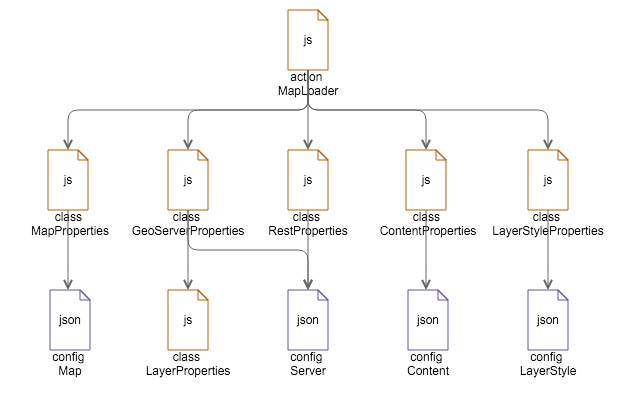
\includegraphics[width=12cm]{img/c02-application/png/app-class-loading.png}
  \caption{Loading JSON and Classes}
\end{figure}

\begin {itemize}
  \item classMapProperties: Retrieves all information about the map contained in the file configMap.json
  \item classGeoServerProperties: Retrieves all information relating to GeoServer contained in the file configServer.json
  \item classRestProperties: Retrieves all information related to the REST API contained in the file configServer.json
  \item classContentProperties: Retrieves all information about Popup content to be displayed above the map in the file configContent.json
  \item classLayerStyleProperties: Retrieves all information about layers contained in the file configLayerStyle.json
  \item classLayerProperties: This class does not depend on a configuration file, it allows to structure a Layer with attributes allowing interractions between the map and the table of contents (TOC). An object from this class will then have a name, an alias, a position, a type layer, a URL to the layer on the GeoServer and map item to display.
\end {itemize}


%%%%%%%%%%%%%%%%%%%%%%%%%%%%%%%%%%%%%%%%%%%%%%%%%%%%%%%%%%%%%%%%%%%%%%%%%%%%%%

% FR
%\subsubsection{Evènements}

% EN
\subsubsection{Events}

% FR
% Le coeur de l'application est concentrée dans des fichiers Javascript préfixés par ``action...''. Chacun de ces fichiers, triés par thème, permet de générer le contenu de la carte. Dans nos sources, les fichiers sont chargés dans l'ordre suivant afin d'obtenir toutes les fonctions nécessaires avant de charger la totalité de la carte : 

% \begin {itemize}
%   \item Les fichiers Javascript des différents Frameworks (jQuery, Bootstrap, Extensions de Bootstrap, Leaflet, Extensions de Leaflet).
%   \item Les fichiers de classes associés aux configurations JSON du paragraphe précédent.
%   \item actionPopup : Ce fichier contient les fonctions relatives aux popup renseignées dans le fichier de configuration JSON des Popup. En effet, chaque popup dispose de ses fonctions, de ses interractions avec la carte et de ses spécificités. Parmis ces fonctions, nous chargeons également le contenu HTML des popup qui seront au-dessus de la carte.
%   \item actionGeoServerLayers : Ce fichier contient les fonctions relatives aux accès GeoServer, aux layers, à leur contenus et tout ce qui s'y rapproche, notamment la récupération des couches de la TOC, la gestion des styles et des bulles d'informations.
%   \item actionMapLoader : Ce fichier est le fichier central de toute l'application, il charge tout les composants nécessaires. Dans un premier temps il se doit de tester la connexion serveur, puis de charger toutes les classes associés aux fichiers JSON, génère les boutons de popup et d'action, récupère les couches GéoServer pour générer la TOC et les afficher sur la carte. Le fichier contient également le rafraichissement de la carte pour chaque déplacement et les variables globales utilisées dans les autres scripts.
% \end {itemize}

% EN
The core of the application is concentrated in Javascript files prefixed with ``action...''. Each of the data sorted by theme, to generate the contents of the map. In our sources, the files are loaded in the following order to obtain all the necessary functions before loading the entire map:

\begin {itemize}
  \item Javascript files of different frameworks (jQuery, Bootstrap, bootstrap extensions, Leaflet, Leaflet Extensions).
  \item Class files associated with JSON configurations of the preceding paragraph.
  \item actionPopup: This file contains the related functions indicated in the popup JSON configuration file. Indeed, every popup has its functions, its interractions with the map and its specificities. Among these functions, we also take care of the HTML content that will show popup over the map.
  \item actionGeoServerLayers: This file contains the functions relating to GeoServer access to layers, their contents and all that it brings, including the recovery of layers of the TOC, management styles and tooltip information.
  \item actionMapLoader : This file is the main file from our application, it loads all the necessary components. At first it should test the server connection, then load all classes associated with JSON files, generates the popup buttons and actions, recovers GeoServer layers to generate the TOC and display them on the map. The file also contains the refresh map for each move and global variables used in other scripts.
\end {itemize}

% \begin{lstlisting}[language=JavaScript]
% % Code here
% \end{lstlisting}

\begin{figure}[ht]
  \centering
  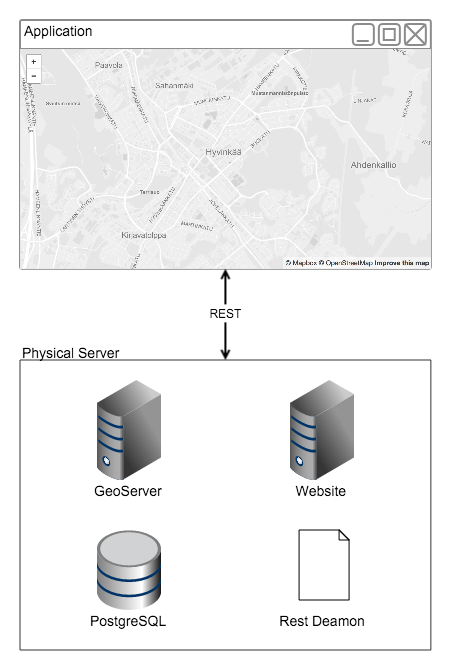
\includegraphics[width=9cm]{img/c02-application/png/app-server-interact.png}
  \caption{Interaction between the application and the server}
\end{figure}








